\chapter{Finite differences in 2D}\label{chap: finite diff 2d}

In this chapter, we study the numerical solution of the Dirichlet boundary-value 
problem for the Poisson equation. Let $\Omega$ be a bounded, open subset 
of~$\mathbb{R}^2$, with a piecewise smooth boundary~$\Gamma=\partial\Omega$.  
Given suitable functions $f(x,y)$~and $g(x,y)$, we see $u=u(x,y)$ satisfying
\begin{equation}\label{eq: Poisson bvp}
\begin{aligned}
-\nabla^2u&=f(x,y)&&\text{for $(x,y)\in\Omega$,}\\
u&=g(x,y)&&\text{for $(x,y)\in\Gamma$.}
\end{aligned}
\end{equation}
Here, the \emph{Laplacian} is the second-order elliptic differential operator
defined by
\[
\nabla^2 u=\nabla\cdot(\nabla u)=\frac{\partial^2u}{\partial x^2}
    +\frac{\partial^2u}{\partial y^2}.
\]

\section{Maximum principle}

\section{Five-point difference scheme}
For simplicity, we now restrict our attention to the case when the spatial 
domain is a rectangle,
\[
\Omega=(0,L_x)\times(0,L_y).
\]
To set up the spatial finite difference grid, we fix positive integers $P$~and 
$Q$, define the step sizes
\[
\Delta x=\frac{L_x}{P}\quad\text{and}\quad\Delta y=\frac{L_y}{Q},
\]
and define the grid points
\[
(x_p,y_q)=(p\,\Delta x,q\,\Delta y)
\quad\text{for $0\le p\le P$ and $0\le q\le Q$.}
\]
Our is to compute $U_{p,q}\approx u(x_p,y_q)$ where $u$ is the solution 
of~\eqref{eq: Poisson bvp}.

Let $\delta_x^2$~and $\delta_y^2$ denote the second-order, central difference 
operators in the $x$- and $y$-directions, respectively; that is,
\[
\delta_x^2u(x,y)=\frac{u(x+\Delta x,y)-2u(x,y)+u(x-\Delta x,y)}{\Delta x^2}
    =\frac{\partial^2u}{\partial x^2}+O(\Delta x^2)
\]
and
\[
\delta_y^2u(x,y)=\frac{u(x,y+\Delta y)-2u(x,y)+u(x,y-\Delta y)}{\Delta x^2}
    =\frac{\partial^2u}{\partial y^2}+O(\Delta y^2).
\]
We also write
\[
\delta_x^2U_{pq}=\frac{U_{p+1,q}-2U_{p,q}+U_{p-1,q}}{\Delta x^2}
\quad\text{and}\quad
\delta_y^2U_{pq}=\frac{U_{p,q}-2U_{p,q}+U_{p,q-1}}{\Delta y^2}.
\]
With this notation, our finite difference scheme can be written compactly as
\begin{equation}\label{eq: 5-pt Poisson}
\begin{aligned}
-\bigl(\delta_x^2U_{p,q}+\delta_y^2U_{p,q}\bigr)&=f_{p,q}
    &&\text{for $(x_p,y_q)\in\Omega$,}\\
U_{p,q}&=g_{p,q}&&\text{for $(x_p,y_q)\in\Gamma$,}
\end{aligned}
\end{equation}
with the obvious abbreviations $f_{p,q}=f(x_p,y_q)$~and $g_{p,q}=g(x_p,y_q)$.
Notice that $(x_p,y_q)\in\Omega$ for $1\le p\le P-1$ and $1\le q\le Q-1$, so 
there are 
\[
M=(P-1)(Q-1)
\]
unknown values of~$U_{p,q}$ at the interior grid points.  The remaining
$(P+1)(Q+1)-M=2P+2Q$ values are given directly by the Dirichlet boundary 
condition.  The finite difference approximation provides one equation for 
each interior grid points, and hence one equation for each unknown, to yield an 
$M\times M$~linear system.  Figure~\ref{fig: 5-pt stencil} shows the stencil 
for the scheme, which involes 5~grid points: $(x_p,y_q)$ and its four nearest 
neighbours $(x_{p-1},y_q)$, $(x_{p+1},y_q)$, $(x_{p,q-1})$~and 
$(x_p,y_{q+1})$.

\begin{figure}
\caption{Five-point finite difference stencil for the discrete Poisson 
equation~\eqref{eq: 5-pt Poisson}.}\label{fig: 5-pt stencil}
\begin{center}
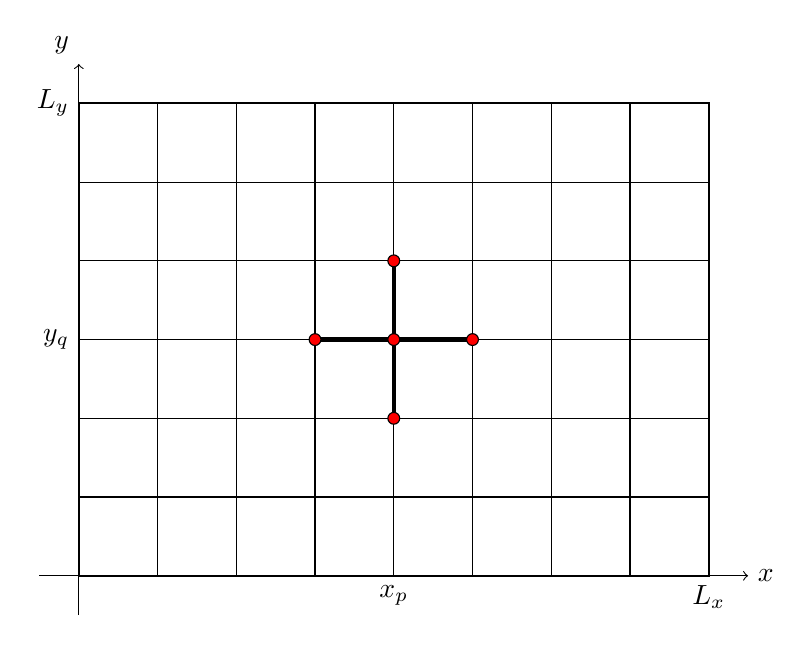
\begin{tikzpicture}[scale=0.5]
\draw[->] (-1,0) -- (17,0);
\node[right] at (17,0) {$x$};
\node[below] at (8,0) {$x_p$};
\draw[->] (0,-1) -- (0,13);
\node[above left] at (0,13) {$y$};
\node[left] at (0,6) {$y_q$};
\foreach \x in {2, 4, ..., 14}
    \draw[thin] (\x,0) -- (\x,12);
\foreach \y in {2, 4, ..., 10}
    \draw[thin] (0,\y) -- (16,\y);
\draw[ultra thick] (8,4) -- (8,8);
\draw[ultra thick] (6,6) -- (10,6);
\draw[fill=red] (8,4)  circle (0.15cm);
\draw[fill=red] (8,6)  circle (0.15cm);
\draw[fill=red] (8,8)  circle (0.15cm);
\draw[fill=red] (6,6) circle (0.15cm);
\draw[fill=red] (10,6) circle (0.15cm);
\node[below] at (16,0) {$L_x$};
\node[left]  at (0,12) {$L_y$};
\draw[thick] (0,0) -- (16,0) -- (16,12) -- (0,12) -- (0,0);
\end{tikzpicture}
\end{center}
\end{figure}

To describe the $M\times M$ system explicitly, we need to arrange the 
unknowns~$U_{p,q}$ into a column vector of length~$M$.  A standard approach is 
to think of the $U_{p,q}$ as the entries of a $(P-1)\times(Q-1)$ matrix and use 
\emph{column-major ordering}, so that
\begin{equation}\label{eq: column-major}
U_j=U_{p,q}\quad
\text{where $j=p+(q-1)(P-1)$ for $1\le p\le P-1$ and $1\le q\le Q-1$.}
\end{equation}
The right-hand sides $f_{p,q}$ are arranged in the same way.  

\begin{example}\label{example: 5-pt matrix}
Suppose $P=5$ and $Q=4$, with $\Delta x=h=\Delta y$.  The finite difference 
equation is then
\[
-\frac{1}{h^2}\bigl(U_{p+1,q}-2U_{p,q}+U_{p-1,q}+U_{p,q+1}2-U_{p,q}+U_{p,q-1}
    \bigr)=f_{p,q},
\]
or equivalently,
\[
\frac{1}{h^2}\bigl(-U_{p,q-1}-U_{p-1,q}+4U_{p,q}-U_{p+1,q}-U_{p,q+1}\bigr)
    =f_{p,q}.
\]
When $p=1$~and $q=3$,
\[
\frac{1}{h^2}\bigl(-U_{1,2}-U_{0,3}+4U_{1,3}-U_{2,3}-U_{1,4}\bigr)
    =f_{1,3},
\]
and the boundary conditions give $U_{0,3}=g_{0,3}$~and $U_{1,4}=g_{1,4}$, so
\[
\frac{1}{h^2}\bigl(-U_{1,2}+4U_{1,3}-U_{2,3}\bigr)
    =f_{1,3}+\frac{1}{h^2}\bigl(g_{0,3}+g_{1,4}\bigr).
\]
Using column-major ordering~\eqref{eq: column-major} with~$P=5$, we have
$U_5=U_{1,2}$, $U_9=U_{1,3}$~and $U_{10}=U_{2,3}$ so the $9$th equation is
\[
\frac{1}{h^2}\bigl(-U_5+4U_9-U_{10}\bigr)=f_9
    +\frac{1}{h^2}\bigl(g_{0,3}+g_{1,4}\bigr).
\]
Figure~\ref{fig: 5-pt matrix} shows the complete $12\times12$ linear system.
\end{example}

\begin{figure}
\caption{The $12\times12$ linear system from 
Example~\ref{example: 5-pt matrix}.}\label{fig: 5-pt matrix}
\begin{gather*}
\frac{1}{h^2}
\left[\begin{array}{cccc|cccc|cccc}
 4&-1& 0& 0&  -1& 0& 0& 0&   0& 0& 0& 0\\
-1& 4&-1& 0&   0&-1& 0& 0&   0& 0& 0& 0\\
 0&-1& 4&-1&   0& 0&-1& 0&   0& 0& 0& 0\\
 0& 0&-1& 4&   0& 0& 0&-1&   0& 0& 0& 0\\
\hline
-1& 0& 0& 0&   4&-1& 0& 0&  -1& 0& 0& 0\\
 0&-1& 0& 0&  -1& 4&-1& 0&   0&-1& 0& 0\\
 0& 0&-1& 0&   0&-1& 4&-1&   0& 0&-1& 0\\
 0& 0& 0&-1&   0& 0&-1& 4&   0& 0& 0&-1\\
\hline
 0& 0& 0& 0&  -1& 0& 0& 0&   4&-1& 0& 0\\
 0& 0& 0& 0&   0&-1& 0& 0&  -1& 4&-1& 0\\
 0& 0& 0& 0&   0& 0&-1& 0&   0&-1& 4&-1\\
 0& 0& 0& 0&   0& 0& 0&-1&   0& 0&-1& 4
\end{array}\right]
\left[\begin{array}{c}
U_{1,1}\\ U_{2,1}\\ U_{3,1}\\ U_{4,1}\\ 
\hline
U_{1,2}\\ U_{2,2}\\ U_{3,2}\\ U_{4,2}\\                
\hline
U_{1,3}\\ U_{2,3}\\ U_{3,3}\\ U_{4,3}                
\end{array}\right]\\
=\left[\begin{array}{c}
f_{1,1}\\ f_{2,1}\\ f_{3,1}\\ f_{4,1}\\                
\hline
f_{1,2}\\ f_{2,2}\\ f_{3,2}\\ f_{4,2}\\                
\hline
f_{1,3}\\ f_{2,3}\\ f_{3,3}\\ f_{4,3}                
\end{array}\right]
+\frac{1}{h^2}\left[\begin{array}{c}
g_{01}+g_{10}\\ g_{20}\\ g_{30}\\ g_{40}+g_{51}\\ \hline
g_{02}       \\ 0     \\ 0     \\ g_{52}\\ \hline
g_{03}+g_{14}\\ g_{24}\\ g_{34}\\ g_{44}+g_{53}
\end{array}\right].
\end{gather*}
\end{figure}

\section{Matrix structure}
The structure of the matrix arising from the discrete Poisson 
problem~\eqref{eq: 5-pt Poisson} can be understood more easily with the help of 
the following concept.

\begin{definition}
Given matrices
$\boldsymbol{A}\in\mathbb{R}^{M\times N}$~and 
$\boldsymbol{B}\in\mathbb{R}^{P\times Q}$, the \emph{Kronecker product} 
$\boldsymbol{A}\otimes\boldsymbol{B}\in\mathbb{R}^{(MP)\times(NQ)}$ 
is the $M\times N$ block matrix whose $ij$-block equals $a_{ji}\boldsymbol{B}$,
that is,
\[
\boldsymbol{A}\otimes\boldsymbol{B}=\begin{bmatrix}
a_{11}\boldsymbol{B}&a_{12}\boldsymbol{B}&\cdots&a_{1N}\boldsymbol{B}\\
a_{21}\boldsymbol{B}&a_{22}\boldsymbol{B}&\cdots&a_{2N}\boldsymbol{B}\\
              \vdots&              \vdots&\ddots&              \vdots\\
a_{M1}\boldsymbol{B}&a_{M2}\boldsymbol{B}&\cdots&a_{MN}\boldsymbol{B}
\end{bmatrix}.
\]
\end{definition}

\begin{example}\label{example: Kronecker product}
If
\[
\boldsymbol{A}=\begin{bmatrix}1&3\\ 2&4\end{bmatrix}
\quad\text{and}\quad
\boldsymbol{B}=\begin{bmatrix}1&0&-3\\ -2&1&-1\end{bmatrix}
\]
then
\[
\boldsymbol{A}\otimes\boldsymbol{B}
=\begin{bmatrix}
 \boldsymbol{B}&3\boldsymbol{B}\\
2\boldsymbol{B}&4\boldsymbol{B} 
\end{bmatrix}
=\left[\begin{array}{ccc|ccc}
 1& 0&-3& 3& 0&-9\\
-2& 1&-1&-6& 3&-3\\             
\hline
 2& 0&-6& 4& 0&-12\\
-4& 2&-2&-8& 4&-4
\end{array}\right].
\]
\end{example}

The next theorem gives a key relation between the Kronecker product and the 
ordinary matrix product.

\begin{theorem}\label{thm: Kronecker A B C D}
If $\boldsymbol{A}\in\mathbb{R}^{M\times N}$,
$\boldsymbol{B}\in\mathbb{R}^{P\times Q}$,
$\boldsymbol{C}\in\mathbb{R}^{N\times R}$~and
$\boldsymbol{D}\in\mathbb{R}^{Q\times S}$, then
\[
(\boldsymbol{A}\otimes\boldsymbol{B})(\boldsymbol{C}\otimes\boldsymbol{D})
=(\boldsymbol{A}\boldsymbol{C})\otimes(\boldsymbol{B}\boldsymbol{D}).
\]
\end{theorem}
\begin{proof}
The $ij$-block of 
$(\boldsymbol{A}\otimes\boldsymbol{B})(\boldsymbol{C}\otimes\boldsymbol{D})$ 
equals
\[
\sum_{k=1}^N(a_{ik}\boldsymbol{B})(c_{kj}\boldsymbol{D})
    =\biggl(\sum_{k=1}^Na_{ik}c_{kj}\biggr)(\boldsymbol{B}\boldsymbol{D})
    =(\boldsymbol{A}\boldsymbol{C})_{ij}(\boldsymbol{B}\boldsymbol{D}),
\]
which is also the $ij$-block of
$(\boldsymbol{A}\boldsymbol{C})\otimes(\boldsymbol{B}\boldsymbol{D})$.
\end{proof}

\begin{example}
\newcommand{\bs}[1]{\boldsymbol{#1}}
With $\boldsymbol{A}$~and $\boldsymbol{B}$ as in 
Example~\ref{example: Kronecker product}, and with
\[
\boldsymbol{C}=\begin{bmatrix}1&-1&3\\ 5&0&3\end{bmatrix}
\quad\text{and}\quad
\boldsymbol{D}=\begin{bmatrix}1&0&7\\ 0&-4&1\\ 2&3&9\end{bmatrix},
\]
we have
\[
(\bs{A}\otimes\bs{B})(\bs{C}\otimes\bs{D})
    =\begin{bmatrix}
 \bs{B}&3\bs{B}\\
2\bs{B}&4\bs{B}\end{bmatrix}
\begin{bmatrix}
 \bs{D}&-\bs{D}&3\bs{D}\\
5\bs{D}& \bs{0}&3\bs{D}
\end{bmatrix}
=\begin{bmatrix}
16\bs{B}\bs{D}& -\bs{B}\bs{D}&12\bs{B}\bs{D}\\
22\bs{B}\bs{D}&-2\bs{B}\bs{D}&18\bs{B}\bs{D}
\end{bmatrix}
\]
which is the same matrix as
\[
(\bs{A}\bs{C})\otimes(\bs{B}\bs{D})
=\left(\begin{bmatrix}1&3\\ 2&4\end{bmatrix}
\begin{bmatrix}1&-1&3\\ 5&0&3\end{bmatrix}\right)\otimes(\bs{B}\bs{D})
=\begin{bmatrix}16&-1&12\\ 22&-2&18\end{bmatrix}\otimes(\bs{B}\bs{D}).
\]
\end{example}

The Kronecker product makes sense for vector operands, if we identify an
$N$-dimensional row vector with a $1\times N$~matrix, and identify an 
$N$-dimensional column vector with an $N\times1$~matrix.  Suppose that
\[
\newcommand{\bs}[1]{\boldsymbol{#1}}
\bs{U}=\bs{w}\otimes\bs{v}
    =\begin{bmatrix}w_1\bs{v}\\ w_2\bs{v}\\ \vdots\\ w_{Q-1}\bs{v}\end{bmatrix}
\quad\text{for $\bs{v}\in\mathbb{R}^{P-1}$ and $\bs{w}\in\mathbb{R}^{Q-1}$,}
\]
so that
\[
U_j=U_{p,q}=v_pw_q\quad\text{where $j=p+(q-1)(P-1)$,}
\]
for $1\le p\le P-1$ and $1\le q\le Q-1$.  Define
\[
\boldsymbol{A}_x=\frac{1}{\Delta x^2}\begin{bmatrix}
 2&    -1&      &      &\\
-1&     2&    -1&      &\\
  &\ddots&\ddots&\ddots&\\
  &      &    -1&     2&-1\\
  &      &      &    -1& 2\end{bmatrix}\in\mathbb{R}^{(P-1)\times(P-1)}
\]
and
\[
\boldsymbol{A}_y=\frac{1}{\Delta y^2}\begin{bmatrix}
 2&    -1&      &      &\\
-1&     2&    -1&      &\\
  &\ddots&\ddots&\ddots&\\
  &      &    -1&     2&-1\\
  &      &      &    -1& 2\end{bmatrix}\in\mathbb{R}^{(Q-1)\times(Q-1)},
\]
so that
\begin{equation}\label{eq: delta x y separable}
-\delta_x^2U_{p,q}=(\boldsymbol{A}_x\boldsymbol{v})_pw_q
\quad\text{and}\quad
-\delta_y^2U_{p,q}=v_p(\boldsymbol{A}_y\boldsymbol{w})_q,
\end{equation}
if we set $v_0=0=v_P$ and $w_0=0=w_Q$.  These relations correspond to the case 
when $u(x,y)=v(x)w(y)$ so that $-u_{xx}=(-v'')w$~and $u_{yy}=v(-w'')$.

\begin{theorem}
Let
\[
\boldsymbol{A}\boldsymbol{U}=\boldsymbol{f}+\boldsymbol{g}
\]
be the linear system resulting from the discrete Poisson 
problem~\eqref{eq: 5-pt Poisson} scheme~\eqref{eq: 5-pt Poisson}.  Then,
\[
\boldsymbol{A}=\boldsymbol{I}_y\otimes\boldsymbol{A}_x
    +\boldsymbol{A}_y\otimes\boldsymbol{I}_x,
\]
where $\boldsymbol{I}_x$~and $\boldsymbol{I}_y$ are the identity matrices of 
dimension $P-1$~and $Q-1$, respectively.
\end{theorem}
\begin{proof}
We see from \eqref{eq: delta x y separable}~and 
Theorem~\ref{thm: Kronecker A B C D} that
\begin{align*}
\boldsymbol{A}(\boldsymbol{w}\otimes\boldsymbol{v})
    &=\boldsymbol{w}\otimes(\boldsymbol{A}_x\boldsymbol{v})
    +(\boldsymbol{A}_y\boldsymbol{w})\otimes\boldsymbol{v}\\
    &=\bigl(\boldsymbol{I}_y\boldsymbol{w})
        \otimes(\boldsymbol{A}_x\boldsymbol{v})
    +(\boldsymbol{A}_y\boldsymbol{w})
        \otimes(\boldsymbol{I}_x\boldsymbol{v})\\
    &=(\boldsymbol{I}_y\otimes\boldsymbol{A}_x)
        (\boldsymbol{w}\otimes\boldsymbol{v})
    +(\boldsymbol{A}_y\otimes\boldsymbol{I}_x)
        (\boldsymbol{w}\otimes\boldsymbol{v})\\
    &=\bigl(\boldsymbol{I}_y\otimes\boldsymbol{A}_x
    +\boldsymbol{A}_y\otimes\boldsymbol{I}_x\bigr)
        (\boldsymbol{w}\otimes\boldsymbol{v})
\end{align*}
for every $\boldsymbol{v}\in\mathbb{R}^{P-1}$ and 
$\boldsymbol{w}\in\mathbb{R}^{Q-1}$.
\end{proof}




\section{Band Cholesky factorization}

\section{Parabolic problems in 2D}
